\documentclass[10pt,twocolumn]{article}
\usepackage{graphicx}
\usepackage{times}
\usepackage{fancyhdr}
\usepackage{tabularx}
\usepackage{hhline}
\usepackage{color}
\usepackage{alltt}
%\usepackage{draftcopy}
\usepackage{xspace}
%\usepackage{parskip}
\usepackage{url}
\setlength{\voffset}{0in}
\setlength{\hoffset}{0in}
\setlength{\headheight}{0pt}
\setlength{\topmargin}{-.25in}
\setlength{\oddsidemargin}{0in}
\setlength{\evensidemargin}{0in}
\setlength{\textheight}{9in}
\setlength{\textwidth}{6.5in}
\setlength{\headsep}{.25in}
\usepackage{cite}
% \setlength{\columnsep}{0.11in}
%\addtolength{\parskip}{-0.5*\baselineskip}


\pagestyle{plain}

%% The name of the system is....?
\def\Sys{P2\xspace}
\def\Lang{OverLog\xspace}

\renewcommand{\ttdefault}{cmtt}
\newenvironment{overlog}{\begin{alltt}\footnotesize}{\end{alltt}}
\newcommand{\ol}[1]{{\tt\footnotesize#1}}

%\newcommand{\note}[1]{[{\textit{#1}}]}
%\newcommand{\note}[1]{[\textcolor{red}{\textit{#1}}]}
\newcommand{\note}[1]{}


\let\oldthebibliography=\thebibliography
\let\endoldthebibliography=\endthebibliography
\renewenvironment{thebibliography}[1]{%
    \begin{oldthebibliography}{#1}%
    \setlength{\parskip}{0ex}%
    \setlength{\itemsep}{0ex}%
}%
{%
    \end{oldthebibliography}%
}
\bibliographystyle{abbrv}
\markboth{Draft}{Preprint--Please do not redistribute}
\pagestyle{myheadings}


\begin{document}
\title{On-line Debugging of Overlay Networks in \Sys}
\author{Atul Singh, Boon Thau Loo, Petros Maniatis, Timothy Roscoe, Joseph M.\ Hellerstein\\
Rice University, UC Berkeley, and Intel Research Berkeley}
\date{}
\maketitle
\thispagestyle{plain}

\begin{abstract}
We present our vision for the on-line debugging of overlays at multiple
levels of abstraction, as enabled by P2, an overlay development and
deployment framework we are currently building.  We argue that
extracting execution information automatically from a system's logical
specification and its translation to a distributed dataflow, we can
identify and understand bugs at the right level of
abstraction, without modifying the executing system. The resulting
techniques are powerful and promise a less-painful future for overlay
development and debugging.
%{\tiny
%\begin{verbatim}
%$Id: paper.tex,v 1.61 2005/08/02 20:18:52 maniatis Exp $
%\end{verbatim}
%}
\end{abstract}



\section{Introduction}
\label{sec:intro}

Modern networked systems need to track the membership of 
participating nodes and coordinate message delivery among them.  This
task is at the core of Internet routing protocols like BGP and OSPF
but is also needed for networked 
applications like enterprise-scale mail services, peer-to-peer
file-sharing systems, and distributed hash tables.  At the
application-level, this is
the task of an {\em overlay network}.

%% Overlay implementation is hard even for
%% experienced programmers.  It typically follows a multi-step
%% methodology, starting with the invariant
%% properties for the network to maintain, including topology (e.g., low
%% diameter~\cite{rowstron-ngc01}, low 
%% degree~\cite{singh-EW04}), route selection
%% (e.g., route flexibility~\cite{gummadi-sigcomm03}) or even flexible
%% recipient selection~\cite{rowstron-ngc01}.  Next, 
%% the designer must find or invent a distributed algorithm to
%% achieve these properties, e.g. Dijkstra's algorithm for shortest
%% paths, Chord for consistent hashing~\cite{Stoica2003}, or core-based
%% trees for multicast tree construction~\cite{rfc:2189}.  This algorithm
%% must then be translated into a host protocol implementation.
%% The code is typically tested in a simulation or emulation
%% setting~\cite{emulab:website,p2psim:website} 
%% to find and remove bugs. Finally, the system is deployed ``in the
%% wild'', where debugging and monitoring continues online.  The whole
%% process is also generally iterative. 

Overlay implementation is hard even for
experienced programmers.  It typically follows a multi-step
methodology, starting with the invariant
properties for the network to maintain, including topology (e.g., low
diameter or low degree), route selection flexibility, or even flexible
recipient selection.  Next, 
the designer must find or invent a distributed algorithm to
achieve these properties, e.g., Dijkstra's algorithm for shortest
paths or core-based
trees for multicast tree construction.  This algorithm
must then be translated into a host protocol implementation.
The code is typically tested in a simulation or emulation
setting
to find and remove bugs. Finally, the system is deployed ``in the
wild,'' where debugging and monitoring continues on-line.  The whole
process is also generally iterative. 

Bugs can be introduced at each step of this quest,
and finding and fixing bugs in networked systems is a
painstaking process~\cite{jones-04,muir-worlds04}.
Current debugging techniques and tools provide little help
at any of these steps, and essentially no help {\em across} steps.  In
this paper we describe techniques to significantly
improve this state of affairs in \Sys, a network construction system
we are developing~\cite{Loo2005SOSP}.  A key feature of our
work is {\em multi-resolution debugging}: the
ability to specify and execute debugging tasks concurrently at different
levels of abstraction.  

% Multi-resolution system inspection, both for invariant
% monitoring and for execution tracing, can catch problems that strict
% layering can obfuscate~\cite{jones-04}.  Consider, for instance, a
% watchpoint that logs the queue lengths for any queue involved in the
% $k$ highest-latency forwarding paths in an overlay, regardless of a
% queue's layer of abstraction (application, network, system event,
% etc.).

\Sys itself provides an execution
environment that represents overlays at three levels of
abstraction.  Programmers interact with the system at the highest
level, by specifying network protocols {\em declaratively}, via a
declarative logic language called \Lang. 
\Lang is automatically compiled to
a dataflow graph specifying the flow of data -- packets and information
``tuples'' -- among {\em elements}
that perform both network packet handling,
% (much like the Click router toolkit~\cite{click-tocs})
and database-like data operations.  Each element is
a C++ object, and the ``flow'' of data through the graph is handled
by a small event dispatcher in the \Sys runtime.

The debugging and monitoring features we introduce in this paper mirror the
architecture and benefits of \Sys, providing multi-resolution
debugging and monitoring.  High-level  (typically distributed)
invariants or {\em logical watchpoints} can be specified in
\Lang: \Sys translates these into dataflows that run as part of the
execution, raising alerts when a particular condition occurs.
Individual \Lang rules can also be traced to provide a 
logic-level understanding of program behavior.  Mid-level debugging
and monitoring is done by
directly {\em tapping} the dataflow graph, shunting copies of data at
various points to logs or real-time monitoring
elements.  These logs and monitors can be used to trace the
distributed {\em lineage} of messages in the system -- all information
(events, computational outputs) that contributed to the production of
another piece of information.  Finally, at the lowest level, the
programmer can always resort to a traditional code debugger to
investigate the behavior of an individual element or the dataflow
dispatcher itself.  

We stress two important properties that emerge from our debugging
framework.  First, monitoring is done on the 
{\em native specification}, either in \Lang or additional
dataflow elements, and we leverage \Sys's inherent
ability to execute on-line, distributed dataflow: in short, to perform
distributed queries.  This allows on-line continuous querying and
monitoring, logging followed by distributed querying of the
logs, and even monitoring tasks that compare live behavior to
past, logged behavior.  It also allows \Sys  to monitor
other networks, as we discuss briefly in
Section~\ref{sec:design}.  Second, debugging is {\em decoupled from
  program logic}: debugging behaviors, whether specified in
\Lang or explicitly wired into a dataflow graph, tap 
dataflow streams connecting elements; they are decoupled from the
overall shape of the graph and from the details of the element implementations.
Hence, debugging specifications require no 
modification of the core logic of the program: there is no need to go
back to the low-level implementation and intersperse instrumentation
statements into operational code blocks.  This makes it
easy to add debugging rules and ensures that the debugging
logic remains meaningful as the code itself evolves.

% XXX This is more important than just a P2 debugger.  Provided some data
% gathering facilities offered by systems not implemented in P2, we can
% provide a distributed analysis with the P2 debugger.  This analysis is
% more comprehensive the more comprehensive the ``taps'' into the foreign
% system are. XXX

In what follows we present the current, early design for the \Sys
debugging environment.  We give a brief overview of \Sys
(\S~\ref{sec:P2}) to ground the discussion for a debugging usage
scenario demonstrating the features that approximate our vision
(\S~\ref{sec:scenario}). In \S~\ref{sec:design} we present some of the
design challenges and opportunities that lie ahead, as we continue our
work.  We survey related work (\S~\ref{sec:related}) and then
conclude.



% Distributed systems are necessarily complex compared to centralized
% systems.  In typical decentralized settings, such systems must
% self-organize in ``overlays'' --- from low-level routing protocols like
% BGP and OSPF to high-level end-system multicast or consistent hashing
% topologies --- to enable discovery, communication, load
% balancing, and configuration management.
% 
% Implementing these overlays and the distributed systems that employ them
% can be a very challenging task.  In one typical methodology, the designer defines
% a set of invariant properties she wishes to instill into the 
% system such as consistent partitioning of requests~\cite{karger-stoc97}, a low-diameter
% topology~\cite{rowstron-ngc01}, low node in- and
% out-degrees~\cite{singh-EW04}, high
% route flexibility~\cite{gummadi-sigcomm03}, or other similar high-level
% global conditions.  In the next step, the
% designer must identify from the
% literature or develop herself the algorithms that implement
% the desired behavior such as Dijkstra's algorithm for shortest
% path computation, Chord for consistent hashing~\cite{Stoica2003},
% or core-based trees for multicast tree construction~\cite{rfc:2189}. Next comes the
% translation of these algorithms from pseudocode to a programming
% language such as C++.  Then, the code is executed in a 
% controlled simulation or emulation setting~\cite{emulab:website,p2psim:website} and the designer
% attempts to locate and remove bugs. Finally,
% the system is deployed ``in the wild'' and the designer switches to 
% debugging and monitoring the running system.
% 
% Debugging and monitoring such applications is a truly painstaking
% process~\cite{jones-04,muir-worlds04}. Firstly, a human translating the
% high level properties of the
% system to executable code that effects the expected behavior
% can make mistakes.
% An intended global invariant may not match the
% choice of algorithms to achieve it, perhaps because some necessary
% preconditions cannot be assumed or because the local algorithms are
% plainly wrong. Even if the algorithms are correct, their translation to a
% program can be error-prone, resulting in code that diverges from the
% intended logic.
% 
% Secondly, running the system in a distributed setting is inherently difficult and also
% different from emulation or simulation.
% Even if the system correctly matches the intended invariants in
% simulation, it can fail in the wild possibly due to 
% unhandled corner-cases or rare race-conditions.
% 
% Thirdly, few systems are originally designed 
% to ease debugging and monitoring. When
% the unavoidable bugs do pop up, developers must compensate by
% ``patching'' the codebase with logging and assertions, making the system
% difficult to reason about, and potentially introducing new bugs in the process.
% It is telling that despite the plethora
% of overlay algorithms and designs published in the last 6 years, still only a
% (small) handful of production-quality systems exist.  This is truly
% tough work.
% 
% In this paper, we make a case for a development and deployment
% environment that reduces the pain and suffering involved in distributed
% systems debugging, by advocating \emph{high-level watchpoints}, \emph{automated
% support for execution tracing}, \emph{multi-resolution system introspection},
% and \emph{on-line, in-place operation}.  High-level watchpoints bridge the gap
% between local-view algorithmic specifications --- e.g., 
% ``every 10 seconds send a state update to a
% random neighbor'' --- and the global-view intent of that specification
% --- ``use an expander graph to propagate state updates with low latency
% and high fault-tolerance.'' They help identify violations of the
% invariants that designers hope to maintain bottom-up.
% 
% Execution tracing is essential when such monitored invariants are 
% violated.  The designers can learn much inspecting the
% preconditions that lead to the violation, by
% tracing backwards from it to its causes anywhere in the
% system.  Forward tracing from a local event
% that should have resulted in a global
% outcome but did not can reveal a logical disconnect or
% false assumptions about the system's state or environment.
% Automation in execution tracing support eliminates the pesky
% problems occuring when a manually inserted logging statement exports 
% too little information or is itself buggy.
% 
% Multi-resolution system inspection, both for invariant monitoring and for
% execution tracing, can catch problems that strict layering can
% obfuscate~\cite{jones-04}.  Consider, for instance, a watchpoint that
% logs the queue lengths for any queue involved in the $k$ highest-latency
% forwarding paths in an overlay, regardless of a queue's layer of
% abstraction (application, network, system event, etc.).
% 
% Finally, we believe that an \emph{on-line} debugger that allows dynamically
% modifying watchpoints or tracing strategies can intercept unpredictable
% exceptional conditions that are too poorly understood to be reproduced
% in the lab post-mortem.  Wide distribution makes such a task especially
% tricky if the monitor-debug-fix-monitor cycle must include a backhauling
% operation of all relevant information to a central place for inspection
% and evaluation.
% 
% 
% In what follows we present an early design for such an on-line distributed
% debugging environment within the context of \Sys, a framework for the
% rapid, declarative prototyping of overlays~\cite{Loo2005SOSP}.  We briefly
% describe the features of \Sys (\S~\ref{sec:P2}) to ground the discussion
% for a debugging usage scenario demonstrating the features that
% approximate our vision (\S~\ref{sec:scenario}). In \S~\ref{sec:design}
% we present some of the design challenges and opportunities that lie
% ahead, as we continue our work.  We survey related work
% (\S~\ref{sec:related}) and then conclude.
% 





%%%%%%%%%%%%%%%%%%%%%%%%%%%%%%%%%%%%%%%%%%%%%%%%%%%%%%%%%%%%%%%%%%%%%%
\section{\Sys}
\label{sec:P2}

\Sys~\cite{Loo2005SOSP} casts overlay maintenance as 
query processing: the fundamental state of the system, including
links, link weights, policies, and configuration parameters are
represented logically as \emph{relational tables}.  For instance,
out-links can be represented by a table of tuples of the form [my
address, neighbor address, link weight].  The routing tables of the
overlay form a \textit{database view} made up of soft-state
tables (unicast multi-hop routes, multicast neighbors, etc.) derived
from the base facts by distributed continuous queries. 
Overlay operations are, themselves, queries on these tables, often
recursive. 

\Sys expresses queries in \Lang, a variant of the
Datalog language used in deductive databases. A query is a series of deductive
rules of the form [result :- preconditions.], interpreted as ``the
result is true when all preconditions are met.''
For example, in the following:
\begin{overlog}
path(B,C,[B,A]+P,W+Y) :- link(A,B,W),path(A,C,P,Y).
\end{overlog}
the precondition is that the tables named \ol{link} and \ol{path} contain
entries in which the first respective fields match.  When
this occurs, a tuple for \ol{path} is created whose fields are
computed from the input entries. Interpreted logically,
this rule says that if node A has a symmetric network link of weight W
to B, and node A has a path P to node C with cost Y, then node B also
has a path to C formed by prepending the link [B,A] to A's path to
C. The cost of this new path is W+Y.

Globally, this rule can (na\"ively) build
all routing paths 
from all sources to all destinations.  In practice, each individual node
manages only some of each table's tuples.  We 
use the convention that the first field of a tuple denotes where
the tuple lives. When the rule above triggers, the resulting \ol{path}
tuple must be sent to the address in its first field,
where it is inserted in the local \ol{path} table.  For clarity, \Lang
allows link@A(B,W) instead of link(A,B,W).

\Sys automatically translates rules into a
\emph{distributed dataflow} of C++ elements
(much like Click~\cite{click-tocs}) such
as database joins, selections and projections, as well as queues,
multiplexers, demultiplexers, etc.  The rule above is translated to
the dataflow in Figure~\ref{fig:DataFlow}. 
\begin{figure}
\centerline{\includegraphics{DataFlow}}
\caption{Dataflow for the ``all routes'' rule.}
\label{fig:DataFlow}
\end{figure}
The dataflow consists of a network preamble, a number of \emph{rule
strands} produced for each \Lang rule, and a network postamble.  The
preamble is responsible for receiving tuples, unmarshaling them,
queuing them for processing, and then demultiplexing them among the
rule strands. The postamble marshals output tuples and 
sends them to the appropriate destination (first tuple
field). The rule strands are translations of individual \Lang rules
into database query elements.

\noindent {\bf Multi-resolution debugging:}
The \Sys approach offers unique opportunities for the realization of
the debugging functionality envisioned in the introduction, at varying
levels of resolution.  First, as noted above, the design of \Sys as a
declarative dataflow system makes the specification and execution of
high-level distributed ``logical watchpoint'' queries natural.  \Sys
is in essence a distributed query processing system targeted at
network construction and maintenance; while network
monitoring was not its main goal, it is a very natural feature.

Second, \Sys makes it very easy to reason about the logic of the
high-level rule specification, by easily tracing the execution of the
\Lang rules.  In Figure~\ref{fig:DataFlow}, this can be done by
``tapping'' the network inputs, the table lookups, and the outputs of
the shaded rule strands.  In fact, the triggering of each rule is
itself exported automatically as the built-in \Sys table
\ol{exec}, backed by a large in-memory ring buffer, with tuples of the form [NodeID, RuleID, InputTuple,
OutputTuple, OutputDestination, Time].  This table can be queried to
reason about not only the system's current state but its execution
history as well.

Third, once rules are automatically translated into a dataflow of
encapsulated elements, it is possible for the designer to inject
dataflow monitoring logic into the resulting dataflow directly,
without modifying any underlying code.  The designer can tap
individual edges of the underlying dataflow, say between the Join and
Project elements in Figure~\ref{fig:DataFlow}.  Then this ``tap'' can
be either manually connected to other dataflow elements (a la Click),
or it can be exposed as a first-class relational ``view'' in the
system that can be queried in \Lang.  Because the dataflow execution
model schedules elements iff they have data (including event firings)
at their input edges, coarse-grained element-granularity control-flow
events can be traced via taps.  For example, all executions of an
element can be traced by (automatically or manually) inserting taps on
all inputs and outputs of an element.  Similarly one can log all interactions with
the relational tables (e.g., insertions, deletions, expirations, etc.,
from the \ol{path} table), or of elements with their state.
For instance, a queue
element can export its enqueue/dequeue/drop operations in a \ol{queueExec} table with tuples of the form [Node, QueueID, OperationType,
Tuple, Time].  \Sys exposes dataflow
connectivity itself via an \ol{elements} table containing entries for
all dataflow elements in the form [ElementID, ElementType, RuleID],
and a \ol{dataflowLink} table containing entries for all element
connections in the form [SourceElementID, OutputPortNo, Pull/Push,
DestinationElementID, InputPortNo].  System observation at such
granularity can bring out tuning inconsistencies (e.g., a soft state
datum expires before a long delayed update message can refresh it) or
false assumptions (``there are no empty entries in our routing tables
ever'').


Finally, when the debugging process reaches this lowest level of
abstraction without resolving a problem, the designer can go deeper and
inspect the implementation of individual elements in their low-level
programming language (C++). A traditional debugger can be
used, of course, to trace the control-flow within an element.
However, note
that with \Sys the programmer usually needs to look at and modify C++ code only
when debugging individual elements, something we expect to be quite
rare.  This compares favorably
with alternative approaches, where all problems -- including
algorithmic mistakes, anomalies in the distributed state, misuse of
library abstractions, and low-level code errors -- have to be debugged
by looking at the lowest-level single-node operational language
representation.



\section{Usage Scenario}
\label{sec:scenario}

We turn now to a concrete usage example of the
envisioned debugger properties.  We present a scenario involving
P2Chord, an implementation of Chord~\cite{Stoica2003} on \Sys~\cite{Loo2005SOSP}.
For simplicity we abstract some of the rule
details. We assume the following lookup rules.
\begin{overlog}
L1 resp@R(K,SI,E) :- lookup@NI(K,R,E),K in (From,To],
     successor@NI(SI,From,To).
L2 lookup@D(K,R,E) :- lookup@NI(K,R,E),K in (To,From],
     successor@NI(SI,From,To),nextHop@NI(K,D).
\end{overlog}
When node NI receives a lookup by node R for key K
with request identifier E, it can either forward it further, or respond.
If the lookup key lies in the key space (From,To] between NI
and its successor SI, then NI responds directly with its
successor's address in rule L1.  Otherwise, rule L2 looks up the next
hop in NI's \ol{nextHop} table and forwards the lookup to the
resulting node D.


{\bf High-level invariant: Monitoring Routing Consistency} 
Routing consistency is a desirable property of  
Chord. It requires that
only one node be responsible per segment of request space at any time.
We chose consistency
because it is sufficiently involved to demonstrate the strength of our 
debugger, and it is an important property for mission-critical
overlay applications~\cite{MSRPastry-2004}.

Consistent routing is a simple global invariant that would be natural
to specify in \Lang if one wanted to insist that it hold 100\% at all
time.  However, complete consistency of this sort is an unrealistic
goal for a live system undergoing churn.
Instead, it is more typical to sample the state of the network
periodically and test if it is achieving a desired degree of
consistency.  One way to sample consistency is
to lookup key $K$ from different starting nodes at the same time and
to count the received responses that agree.  A consistency violation
occurs when the largest agreeing cluster of responses is smaller than
a minimum threshold, say 50\% of lookups (as per the consistency
definition in Bamboo~\cite{rhea_usenix_2004}).

To sample the consistency invariant in \Lang, we first produce concurrent
lookups from multiple sources.
\begin{overlog}
R0 conProbe@NI(K) :- K=rand(),periodic@NI(t).
R1 conLookup@NI(K,D,E) :- E=rand(),conProbe@NI(K),
     nextHop@NI(K1,D).
R2 lookup@D(K,NI,E)  :- conLookup@NI(K,D,E).
\end{overlog}
Every time period \ol{t}, rule R0 starts a consistency probe with random key
K (\ol{periodic} is a built-in predicate that becomes true at fixed
intervals).  Then rule R1 picks distinct neighbors from the \ol{nextHop}
table and a random request identifier E, and registers a consistency
lookup.  Finally, for every \ol{conLookup} tuple,
rule R2 submits a lookup request to the chosen neighbor node D with a
response returned to the probing node NI.
To collect the responses, rule R3 
registers every response returned whose request
identifier E matches a consistency lookup record:
\begin{overlog}
R3 conResp@NI(K,S,E) :- resp@NI(K,S,E),
     conLookup@NI(K,D,E).
\end{overlog}

To evaluate probe results, we aggregate responses into agreeing
clusters counting the size of each cluster (rule R4), and pick the
largest cluster (R5).  \ol{count<>} is an aggregation operator
counting all responses with common key K and answer S and \ol{max<C>}
finds the maximum cluster size. We also count the probe lookups sent
(R6)\footnote{We omit here for clarity the temporal specification of
  when the clustering occurs for each probe. We use a simple
  fixed-window approach.}.
\begin{overlog}
R4 cluster@NI(K,S,count<>) :- conResp@NI(K,E,S).
R5 maxCluster@NI(K,max<C>) :- cluster@NI(K,S,C).
R6 conLookups@NI(K,count<>) :- conLookup@NI(K,D,E).
\end{overlog}
Finally, we issue an alarm tuple if fewer than 50\% of lookups
resulted in the largest response cluster (R7).
\begin{overlog}
R7 alarm@NI(K) :- conLookups@NI(K,L),
     maxCluster@NI(K,C),C/L<0.5.
\end{overlog}

{\bf High-level Execution tracing}
Given a workable specification of the invariant to be traced,
the next stage for the designer is to understand \emph{why} an alarm
was triggered. She examines the network system states that led to
the alarm, to answer at least the following questions: was it a ``false
alarm,'' possibly due to network instability? did a logical error in the
Chord specification cause this alarm? did some ostensibly correct
logical step produce inexplicable results, meriting deeper perusal?

To perform this forensic analysis, the designer can exploit execution
traces at the granularity of the system's abstract specification.  Using
the \ol{exec} table, she can traverse backwards the
rule execution graph that lead to the alarm's issuance in rule R7. In
fact, she can automate this traversal: the following simple example
sends the execution graph
to a designated node \ol{d}.
\begin{overlog}
T1 backTrace@NI(X,d) :- X=alarm@NI(K).
T2 backTrace@NI(In,D) :- backTrace@OutDest(Out,D),
     exec@NI(Rule,In,Out,OutDest,Time).
T3 report@D(X) :- backTrace@NI(X,D).
\end{overlog}
Rule T1 automatically starts a trace backwards from the alarm tuple when
it is produced (R7), carrying along the eventual destination node
\ol{d}.  Rule T2 traverses recursively each 
\ol{exec} tuple whose output matches the currently traversed tuple to
its input.  Rule T3 sends a copy of every traversed \ol{exec} tuple to
the originally-designated node (specified as \ol{d} in T1).  By appropriately modifying rule T2, more
complex traversal tasks can be performed to identify suspect rule
execution steps, to prune uninteresting graph sections, to store the
graph persistently for prolonged inspection, or for even more
sophisticated execution graph analyses.

Similar rules enable forward execution tracing -- i.e., identifying
all ``downstream'' facts that resulted from the presence of a given
fact. This can be of particular use in pinpointing the cause behind
the {\em absence} of an expected fact downstream.  During actual
P2Chord development, such forward tracing revealed that some probe
lookups were dropped after a few forwarding hops for no apparent
reason. As we describe next, deeper inspection revealed stale routing
entries that caused lookup messages to be sent to dead hosts.




{\bf Building block introspection}
When rule execution tracing locates a suspect step that seems
logically correct, deeper inspection of how that step is implemented
is warranted. For instance, in Figure~\ref{fig:DataFlow}, the top rule
strand may not trigger because the Network is congested and cannot
take the rule's output: it may trigger, but its output is dropped by
the ``Queue'' element upon arrival at its destination; or, it may
trigger and, even though after delivery the produced \ol{path} tuple
is stored in the table, it expires before it can be used for further
rule invocations.


In such cases, the designer will have to trace the execution of the
system at dataflow granularity, using tables such as \ol{queueExec} and
\ol{dataflowLink}.  Conveniently, rules for execution tracing can mix
and match levels of abstraction to express sophisticated logic.  In the
consistency example, while debugging lookups that returned no responses,
the designer may wish to peruse recent queue drop operations in rule
executions that appear at the ``fringe'' of the forward execution graph,
that is, at which forward execution stops.  This might reveal that a
timing mistake is causing routing state to expire prematurely, or might
in turn show that state refreshes are delayed somewhere else in the
execution history of the system.

As with rule-level execution tracing, debugging at the granularity of dataflow
components may not explicate or otherwise fix a bug.  At this stage the designer may have to look at
dataflow element implementations (for instance in C++)
to understand and amend the inexplicable behavior.
Fortunately, element inputs and state that result in suspect outputs are
readily available in the execution history and can be packaged as
unit tests for the benefits of future regression testing of the system.

{\bf Early experience:} 
We have already found our debugger to be useful in debugging the churn
handling rules in P2Chord.  
%% Each node maintains a list of nodes:successor and 
%% predecessor~\footnote{Successor is next node if ring is traversed in
%% cyclic order, while predecessor is next one if traversed in
%% anti-cyclic order. We maintain more than one successor for
%% fault-tolerance, and the closest successor to the local node is its
%% bestSuccessor.}.  
During stabilization periods, each node exchanges
its successor set with its predecessor and successor
nodes. Also, it periodically sends ``keep-alives'' to
its list of nodes, regarding as failed those from which it does not
receive a timely response. 
We observed that certain {\tt lookup} messages were not reaching the
destination. Tracing forward from the initiator of such messages, we
observed that some nodes were forwarding the message to a dead
successor even though it had already been detected as dead.  Observing
updates to the successor table revealed that dead nodes reappeared in the
successor set after they had been declared dead and removed. Tracing
at rule level backwards from the ``undead'' successor entry, we
discovered an execution cycle: a node A found its successor B
dead, updating its successor to C; C during a later stabilization sent
its dead predecessor B back to A without checking it for liveness.
%% (as shown in Figure~\ref{fig:debug-high}).  
This identified a logical
error where our rules did not send ``keep-alive'' messages to the
predecessor nodes, causing a dead predecessor (node B) to
be exchanged during stabilization periods. 

Although a persistent
designer could have found the same bug by manually inserting printing
statements, staring at C++ code, and poring over logs, our automated
tools simplified and sped up this process without touching the
``source'' code of the debugged system.



\if 0
\begin{figure}
\centering
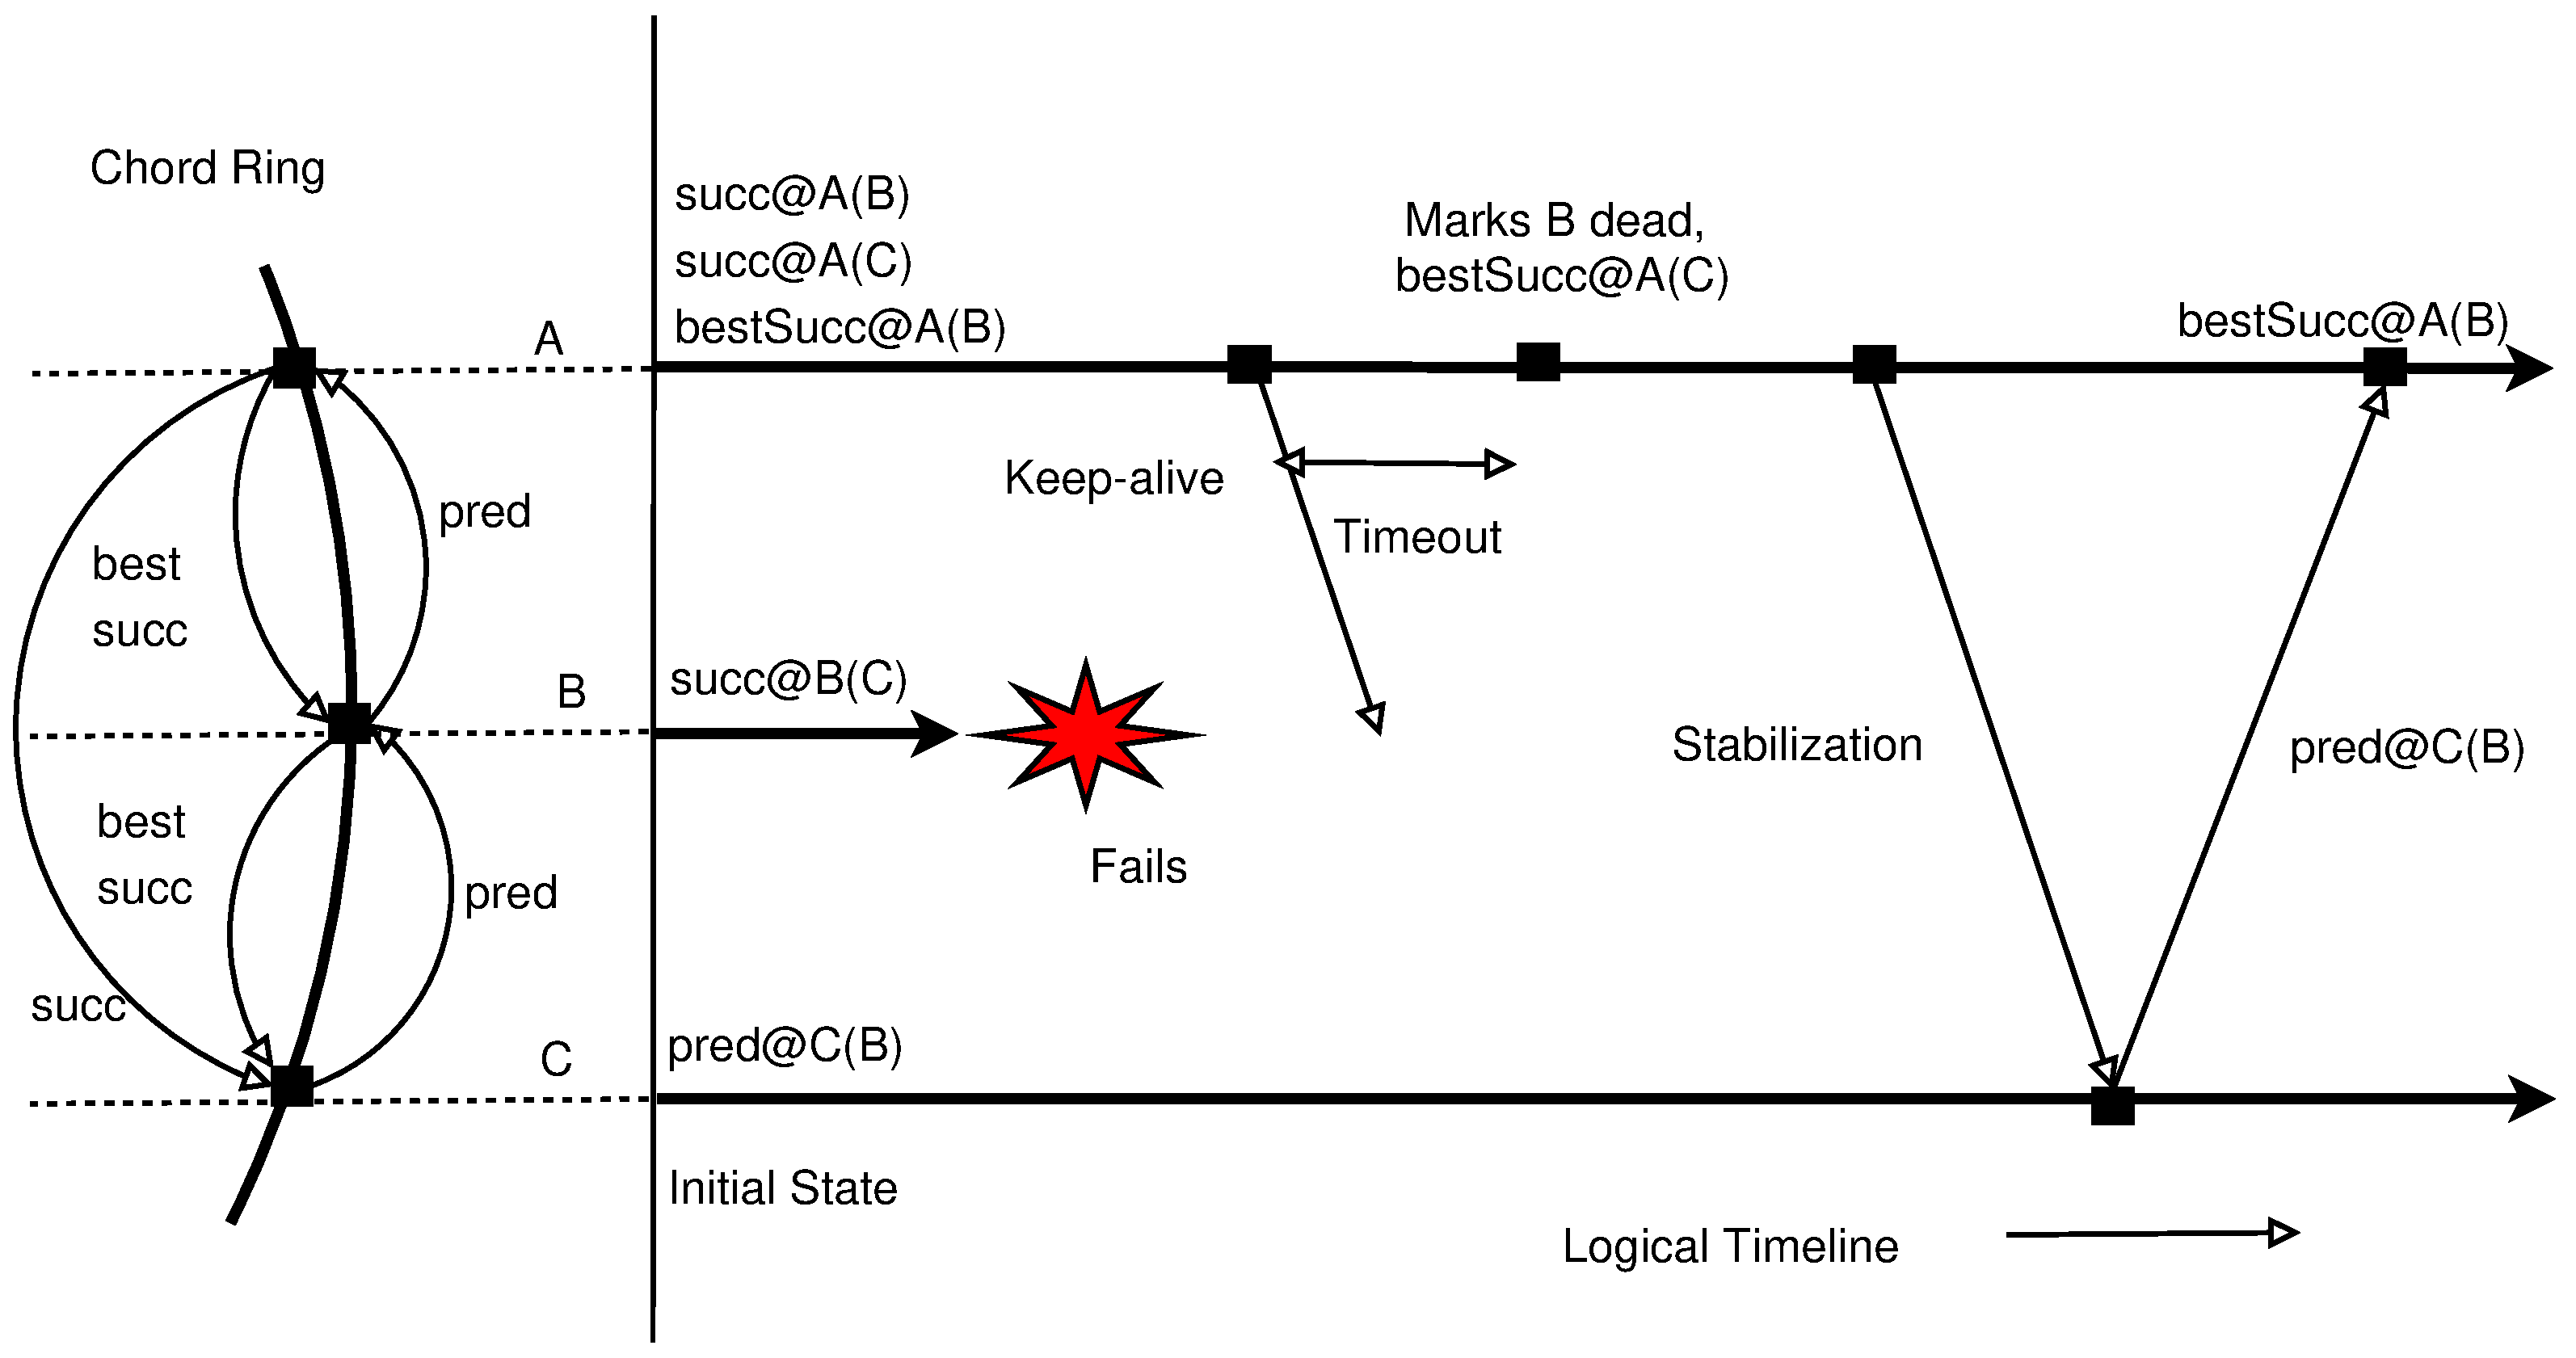
\includegraphics[width=3in]{debug2.eps}
\caption{A simplified, high level view of events depicting the error we had in our rules which 
caused a dead node to be passed around during stabilization periods.}
\label{fig:debug-high}
\end{figure}
\fi

\if 0
\note{Atul to gussy this up somewhat to highlight this paragraph as a
  separate discussion, and to explain how rules would have helped
  detect this problem (had they existed at the time.)}


In our early experience with \Sys debugging features, we used
multi-level tracing to understand why some consistency lookups were
sent to dead hosts. Our implicit assumption had been that
soft-state maintenance of routing tables would evict entries to dead
hosts since no keep-alives refreshed them. We were proven wrong when
dataflow tracing of storage elements revealed that 
entries for dead nodes reappeared in soft-state tables after they had
originally expired. Resuming rule tracing backwards from the ``undead'' routing entries we
discovered an execution cycle: a Chord node gossiped an
almost-expired routing entry to a successor (as per Chord's
stabilization), then expired it, but received it again from the same
successor during the next stabilization exchange and, as a result,
reinstated it after death.  Although a persistent designer could have
found the same bug by manually inserting printing statements, staring at
C++ code, and poring over logs, our automated tools simplified and sped
up this process without touching the ``source'' code of the debugged
system. \note{P: Does this explanation make sense?  I removed the figure
  after rewriting the text.}
\fi


\section{Design Challenges}
\label{sec:design}

The promise of debugging an overlay network at multiple levels of abstraction with a
distributed query processor is very exciting.  Overlays developed with
\Sys gain this benefit without
the need for custom debugging-specific machinery.  Instead, high-level
specifications of debugging queries in \Lang can inspect the running
system and its execution history to pinpoint specific problems.
However, the road ahead towards realizing
this promise poses interesting design challenges.
We
outline some of these below, as well as our initial plans for
tackling them in \Sys.

{\bf Accuracy vs.\ overhead} Complex debugging may directly perturb an
executing application by lengthening event queues, increasing network
usage, stealing away CPU cycles, and consuming storage for extra tables.
A tricky balance must be found among the application's need to make
timely progress under stress and the debugger's need for comprehensive
yet accurate information on the unperturbed running application.
Preferential scheduling and execution of application tasks over
debugging tasks when accuracy is of paramount importance, or vice versa
when immediate comprehensive introspection is the primary goal, might be
a fruitful avenue to explore.

{\bf Usability} Arbitrary execution tracing of a complex running system
can result in a staggering amount of information to inspect.  To be
usable, any debugging facility must help designers to mine the wealth of
available information even when they do not know what they are looking
for.  Tools for interactive clustering, filtering, and refactoring
distributed debugging information may be essential in extracting the
full power of these facilities. Similarly, identifying the appropriate
visual metaphors that present designers with an intuitive
approximation of the system's behavior is certainly non trivial. Given the data-centric
programming paradigm taken in \Sys, techniques from visualizing data
lineage in databases~\cite{Woodruff1997} might prove useful here.

{\bf Linguistic challenges} Specifying breakpoints globally for a
running networked system inspectable at multiple levels of abstraction
can be complex.  In \S~\ref{sec:scenario} we have framed our examples in
\Lang, a rather heavy-handed extension of Datalog still under active
development.  It is fortuitous that in \Sys designers
specify their system in the same language they use to debug it.
However, it is an
open question whether the debugging constructs we use --- in
fact, whether \Lang itself --- are ideal for this task and whether they
offer the flexibility and the intuitive
\emph{feel} that makes debugging overlays tractable.


\section{Related work}
\label{sec:related}

There is a large amount of related work on debugging, monitoring, and testing of 
networked systems.  We limit ourselves to a few exemplars of those
categories of work that are most closely related to ours.

{\bf Monitoring and debugging via database techniques}
Techniques from relational database literature have been used to 
monitor, debug, and manage distributed systems~\cite{conradie-sdne,Hy+,snodgrass-tocs,wolfson-ieee91}.
These proposals typically store logs in centralized
or clustered databases, and provide querying facilities for
information extraction or visualization from stored logs.
However, they concentrate on monitoring tasks and do not inherently
expose execution information of the logic or
implementation of a system.

{\bf Performance debugging}
Inching closer to the execution of a system, recent
proposals~\cite{blackbox-sosp03,magpie-osdi04,causeway-hotos05,chen-path-04}
provide mechanisms to debug the performance properties of networked systems.
They provide mechanisms for tracking the life cycle of an event 
as it passes through different system components (e.g., 
an HTTP request causing a disk access, a page fault, etc.). The gathered information is 
useful for finding causes of anomalous behavior, for capacity 
planning, and detecting performance bugs. In contrast, our proposal
targets protocol bugs and their implications in network overlays,
typically made of smaller-footprint components than a webserver or a
filesystem, which live at a higher level of abstraction than these proposals.

{\bf Debugging configurations or intrusions}
A number of systems attempt to trace the implications of configuration
errors by backtracking inferred causality relationships~\cite{mahajan-sigcomm02,
wang-osdi04,King2003}, or by
mining for events that seem to have effected dramatic changes in a
system~\cite{chronus-osdi04}.  In contrast, we attack a narrower problem
-- overlay networks -- and expose internal causality
relationships among system events that enable sophisticated data
exploration at multiple abstraction levels to pinpoint problems.


{\bf Distributed debuggers}
\if 0
Garcia-Molina et al.~\cite{molina-tose} proposed debugging individual modules
independently before integrating and using tracing (logging) for debugging 
distributed systems. {\bf XXX: Could not get a copy of this on-line - Atul}
\fi
Early work by Bates et al.~\cite{bates-83} proposed an approach to high-level debugging 
that specifies the expected behavior of a network and
compares it to the observed behavior of the implementation.  The
challenge with this approach lies in encoding system behavior from
observable information.  In our approach, the high-level specification
of the system itself facilitates this task, by making explicit
the preconditions and expected output of each algorithmic step.

Harris proposed a virtualized debugger~\cite{harris-EW02} that sandboxes
distributed components in a virtual machine monitor (VMM) to observe and
subsequently replay the external factors affecting system execution
(e.g., processor status, scheduling, etc.). We approach a similar effect
by logging and analyzing the system's execution in the wild.  We
have this luxury because we observe overlays at a level of abstraction
higher than processor flags and interrupts.

Closest to our vision is work by Lin et al.~\cite{wids-hotos05} on an
integrated toolkit for optimizing the implementation and testing of
distributed systems. The authors' hope is to automatically generate
executable code from a high level specification that can run in
simulation as well as real networks.  It is as yet unclear what
high-level abstraction they will use.  In our \Sys implementation, we
use a logic language that compiles to a dataflow implementation,
providing the ability for on-line debugging of the running system at
multiple abstraction levels.



\section{Conclusion and future work}
\label{sec:conclusion}

Debugging an overlay network with P2 appears to offer two clear
advantages. Distributed continuous queries provide a natural
model for checking global properties of a system on-line, rather than
time-consuming offline analysis of logs, and this is a technique that
P2 could apply to any networked system running ``alongside'' it.
However, when combined with P2's logical representation of overlay
protocols as distributed queries themselves, translated into per-node
dataflows, we get an even larger win: the debugging process can now
easily move between layers of abstraction, as illustrated in our early
experience debugging P2Chord. 

Two questions arise from this work.  Firstly, how do we evaluate the
debugger?  Anecdotal evaluation seems to be the norm here, together with
a measurement of performance overhead, but this latter metric is hard
for networked systems.  As a next step, we are implementing
Accordion~\cite{Li2005}, a relatively new P2P protocol providing
bandwidth-efficient routing state on \Sys, to gain experience in
building and debugging a new overlay from scratch.  We plan to report
the experience in building and debugging such a system.

Secondly, can anyone use our debugger?  How effective is P2 when used
for ``sidecar debugging'' of other, more monolithic systems?  We expect
that a developer of an existing overlay network will be able to use P2
to find bugs in a separate implementation not coded in Overlog.  We plan
to connect P2's query processing facilities to the instrumentation
interfaces provided by OpenDHT~\cite{Rhea2005} to investigate this.

{\footnotesize
\bibliography{paper}
}
\end{document}
